\chapter*{Digitalizace obrazových signálů}

Při digitálním zpracování obrazu je dosti často cílem zpracovávat obrazy, které vznikají jako obrazy spojité. Spojitá reprezentace může být žádána také pro výstupy zpracování. Například tehdy, jestliže má být výsledek pozorován člověkem. Pro samotné digitální zpracování obrazu v počítači není však spojitá reprezentace vhodná. Vhodnější je reprezentace diskrétní, kdy je obraz reprezentován spočetnou (v praxi konečnou) množinou nějakých hodnot. Z uvedeného důvodu provádíme před digitálním zpracováním převod obrazu do diskrétní podoby. Říkáme, že obraz vzorkujeme. Dále se při praktické reprezentaci obrazů v počítači vzorky někdy uchovávají jako celočíselné hodnoty. V takových případech pak skutečné úrovně signálu na tyto celočíselné hodnoty převádíme, což nazýváme kvantováním. Po zpracování v digitalizované podobě může být naopak požadována rekonstrukce obrazu do podoby spojité. Problematice vzorkování, kvantování a rekonstrukce je věnována tato kapitola.

\section*{Vzorkování deterministicky popsaných obrazů} \label{sec:vzorkovani_deterministicky_popsanych_signalu}

\begin{figure}[th]
    \begin{center}
        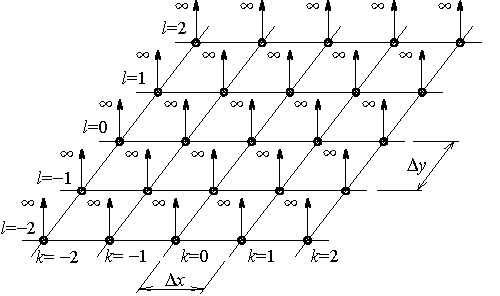
\includegraphics[scale=1.0]{04_digitalizace/images/img_4_1.pdf}
    \end{center}
    \caption{Vzorkovací funkce ve tvaru nekonečného pole Diracových impulzů.}
    \label{img:4_1}
\end{figure}

Předpokládejme, že vzorkujeme vstupní obraz deterministicky popsaný spojitou obrazovou funkcí \textit{f}I(\textit{x},\textit{y}). Aby vztahy, ke kterým dospějeme, vyšly jednoduché, předpokládáme, že je obraz definován nad nekonečnou oblastí. Výsledek vzorkování obrazu je popsán funkcí \textit{f}S(\textit{x},\textit{y}). Jako matematický model vzorkování volíme součin vstupního obrazu se vzorkovací funkcí \textit{s}(\textit{x},\textit{y}). Je tedy

\begin{equation} \label{eq:4_1}
    f_\mathrm{S}(x, y) = f_\mathrm{I}(x, y) s(x, y).
\end{equation}
Jako vzorkovací funkci nejprve zvolíme nekonečné pole Diracových impulzů navzájem vzdálených o $\Delta$\textit{x}, $\Delta$\textit{y} (obr. \ref{img:4_1}). Tato funkce je popsána předpisem

\begin{equation} \label{eq:4_2}
    s(x, y) = \sum\limits_{k=-\infty}^{\infty} \sum\limits_{l=-\infty}^{\infty} \delta(x -k\Delta x, y - l\Delta y).
\end{equation}
Dosazením vztahu \eqref{eq:4_2} do vztahu \eqref{eq:4_1} obdržíme pro \textit{f}$_\mathrm{S}$(\textit{x},\textit{y}) následující předpis

\begin{equation} \label{eq:4_3}
    f_\mathrm{S}(x, y) = \sum\limits_{k=-\infty}^{\infty} \sum\limits_{l=-\infty}^{\infty} f_\mathrm{I}(x, y) \delta(x -k\Delta x, y - l\Delta y).
\end{equation}
Je zřejmé, že ke stanovení funkce \textit{f}$_\mathrm{S}$ podle předpisu \eqref{eq:4_3} stačí znát funkční hodnoty \textit{f}$_\mathrm{I}$ pouze v bodech (\textit{k}$\Delta$\textit{x},\textit{l}$\Delta$\textit{y}). Při praktické realizaci vzorkování jsou proto právě hodnoty \textit{f}$_\mathrm{I}$(\textit{k}$\Delta$\textit{x},\textit{l}$\Delta$\textit{y}) uchovávány. Určeme nyní Fourierovu transformaci \textit{F}$_\mathrm{S}$(\textit{u},\textit{v}) = $\mathscr{F}$\{\textit{f}$_\mathrm{S}$(\textit{x},\textit{y})\} vzorkovaného obrazu \textit{f}$_\mathrm{S}$(\textit{x},\textit{y}). Nechť \textit{F}$_\mathrm{I}$(\textit{u},\textit{v}) = $\mathscr{F}$\{\textit{f}$_\mathrm{I}$(\textit{x},\textit{y})\}, \textit{S}(\textit{u},\textit{v}) = $\mathscr{F}$\{\textit{s}(\textit{x},\textit{y})\} jsou Fourierovy transformace funkcí \textit{f}$_\mathrm{I}$(\textit{x},\textit{y}) a \textit{s}(\textit{x},\textit{y}). Uplatníme-li na obě strany rovnice \eqref{eq:4_1} Fourierovu transformaci a vezmeme-li v úvahu vlastnost \eqref{eq:2_28b}, pak získáme

\begin{equation} \label{eq:4_4}
    F_\mathrm{S}(u, v) = F_\mathrm{I}(u, v) * S(u, v).
\end{equation}
Fourierův obraz nekonečného pole Diracových impulzů jsme vypočetli již dříve v příkladě XXX. Vyšlo

\begin{equation} \label{eq:4_5}
    S(u, v) = \frac{1}{\Delta x \Delta y} \sum\limits_{k=-\infty}^{\infty} \sum\limits_{l=-\infty}^{\infty} \delta \left( u - \frac{k}{\Delta x}, v - \frac{l}{\Delta y} \right).
\end{equation}
Zaveďme frekvence \textit{u}$_\mathrm{S}$, \textit{v}$_\mathrm{S}$ vzorkování jako převrácené hodnoty vzdálenosti vzorků

\begin{equation} \label{eq:4_6}
    u_\mathrm{S} = 1 / \Delta x, \quad v_\mathrm{S} = 1 / \Delta y.
\end{equation}
Dosazením vztahů \eqref{eq:4_5} a \eqref{eq:4_6} do vztahu \eqref{eq:4_4} a rozepsáním konvoluce máme

\begin{equation} \label{eq:4_7}
    F_\mathrm{S}(u, v) = u_\mathrm{S} v_\mathrm{S} \int\limits_{-\infty}^{\infty} \int\limits_{-\infty}^{\infty} F_\mathrm{I}(a, b) \sum\limits_{k=-\infty}^{\infty} \sum\limits_{l=-\infty}^{\infty} \delta(u - a - k u_\mathrm{S}, v - b - l v_\mathrm{S}) \,da\,db.
\end{equation}
Vzájemnou záměnou pořadí integrování a sumace a po úpravě obdržíme

\begin{equation} \label{eq:4_8}
    F_\mathrm{S}(u, v) = u_\mathrm{S} v_\mathrm{S} \sum\limits_{k=-\infty}^{\infty} \sum\limits_{l=-\infty}^{\infty} F_\mathrm{I} (u - k u_\mathrm{S}, v - l v_\mathrm{S}) \,da\,db.
\end{equation}
Nyní jsme došli k významnému závěru: Výraz \eqref{eq:4_8} říká, že frekvenční spektrum \textit{F}$_\mathrm{S}$ vzorkovaného obrazu se skládá ze složek, kterými je spektrum \textit{F}$_\mathrm{I}$ obrazu původního. Složky se periodicky opakují ve vzdálenostech \textit{u}S, \textit{v}S (obr. \ref{img:4_2}) a sčítají. Jak uvidíme později, bude mít pro úspěšnou rekonstrukci obrazu zásadní význam požadavek, aby se jednotlivé složky spektra navzájem nepřekrývaly. Zkoumejme tuto situaci blíže. Předpokládejme, že spektrum vstupního obrazu je omezené - tj., že platí

\begin{figure}[th]
    \begin{center}
        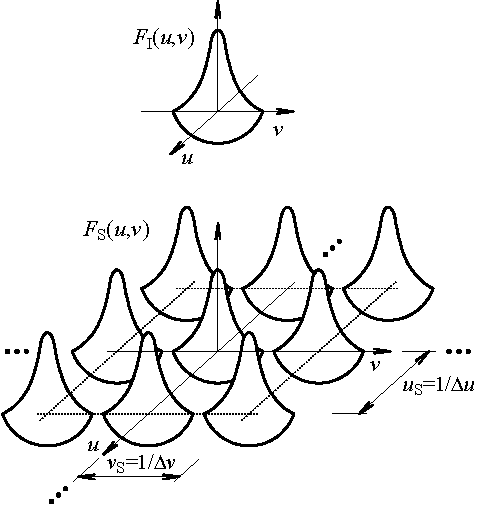
\includegraphics[scale=1.0]{04_digitalizace/images/img_4_2.pdf}
    \end{center}
    \caption{Spektrum původního a vzorkovaného obrazu.}
    \label{img:4_2}
\end{figure}

\begin{equation} \label{eq:4_9}
    F_\mathrm{I}(u, v) = 0, \,\, \mathrm{jestli\check{z}e} \,\, |u| > u_\mathrm{I} \cup |v| > v_\mathrm{I},
\end{equation}
kde hodnoty \textit{u}$_\mathrm{I}$,\textit{v}$_\mathrm{I}$ jsou mezní frekvence vstupního obrazu. Z výrazu \eqref{eq:4_8} vyplývá (viz. též obr. \ref{img:4_2}), že k překrývání složek spektra nedojde za podmínky, že platí nerovnosti

\begin{equation} \label{eq:4_10}
    u_\mathrm{S} \geq 2 u_\mathrm{I}, \quad v_\mathrm{S} \geq 2 v_\mathrm{I}.
\end{equation}
Nyní se budeme zabývat otázkou, za jakých podmínek lze ze vzorkovaného obrazu \textit{f}$_\mathrm{S}$(\textit{x},\textit{y}) vytvořit rekonstruovaný obraz \textit{f}$_\mathrm{R}$(\textit{x},\textit{y}) tak, aby byl shodný se vstupním obrazem \textit{f}I(\textit{x},\textit{y}). Předpokládáme, že rekonstrukci obrazu bude možné provést pomocí nějakého filtru, který proto budeme nazývat filtrem rekonstrukčním. Očekáváme, že rekonstrukční filtr bude lineární a invariantní vůči posunu. Filtr charakterizujeme odezvou \textit{r}(\textit{x},\textit{y}) na Diracův impulz (impulzová charakteristika filtru) a Fourierovou transformací \textit{R}(\textit{u},\textit{v}) této odezvy (frekvenční charakteristika). Tyto funkce však zatím neznáme a chceme je určit.

Z odstavce XXX víme, že obraz na výstupu rekonstrukčního filtru lze stanovit pomocí konvoluce vzorkovaného obrazu a odezvy filtru na Diracův impulz. Je tedy

\begin{equation} \label{eq:4_11}
    f_\mathrm{R}(x, y) = f_\mathrm{S}(x, y) * r(x, y).
\end{equation}
Ve frekvenční doméně pak s ohledem na vlastnost \eqref{eq:2_28a} Fourierovy transformace máme

\begin{equation} \label{eq:4_12}
    F_\mathrm{R}(u, v) = F_\mathrm{S}(u, v) R(u, v).
\end{equation}
Dosadíme-li do vztahu \eqref{eq:4_12} ze vztahu \eqref{eq:4_8}, dostaneme

\begin{equation} \label{eq:4_13}
    F_\mathrm{R}(u, v) = u_\mathrm{S} v_\mathrm{S} R(u, v) \sum\limits_{k=-\infty}^{\infty} \sum\limits_{l=-\infty}^{\infty} F_\mathrm{I} (u - ku_\mathrm{S}, v - lv_\mathrm{S}).
\end{equation}
Předpokládejme, že nedojde k překrývání jednotlivých složek spektra, jak jsme již dříve diskutovali (vztahy \eqref{eq:4_10}). Ze vztahu \eqref{eq:4_13} pak vyplývá, že jestliže navrhneme rekonstrukční filtr tak, aby odfiltroval ty složky spektra, pro které \textit{k} $\neq$ 0, \textit{l} $\neq$ 0, a složku \textit{k} = 0, \textit{l} = 0 naopak propustil, pak \textit{F}$_\mathrm{R}$(\textit{u},\textit{v}) = \textit{F}$_\mathrm{I}$(\textit{u},\textit{v}) a tedy i \textit{f}$_\mathrm{R}$(\textit{x},\textit{y}) = \textit{f}$_\mathrm{I}$(\textit{x},\textit{y}), jak jsme pro rekonstrukci požadovali. Docházíme tedy k závěru, že k optimální rekonstrukci by frekvenční charakteristika rekonstrukčního filtru mohla být např. (obr. \ref{img:4_3})

\begin{equation} \label{eq:4_14} 
    R(u, v) = \left\{
    \begin{array}{cc}
    1, & {\left(|u|\le u_\mathrm{R} \right)\cap \left(|v|\le v_\mathrm{R} \right)} \\
    0, & \mathrm{jinak}
    \end{array}
    \right.,
\end{equation} 
kde \textit{u}$_\mathrm{I}$ $\leq$\textit{u}$_\mathrm{R}$ $\leq$\textit{u}$_\mathrm{S}$/2, \textit{v}$_\mathrm{I}$ $\leq$\textit{v}$_\mathrm{R}$ $\leq$\textit{v}$_\mathrm{S}$/2. (Přesně vzato dává filtr \eqref{eq:4_14} hodnotu \textit{F}$_\mathrm{R}$(\textit{u},\textit{v}) = \textit{u}$_\mathrm{S}$\textit{v}$_\mathrm{S}$\textit{F}$_\mathrm{I}$(\textit{u},\textit{v}), což však nezmenšuje kvalitu rekonstrukce, protože \textit{u}$_\mathrm{S}$\textit{v}$_\mathrm{S}$ je známá konstanta.) Zdůrazněme ještě jednou skutečnost, že podmínkou úspěšné rekonstrukce obrazu je splnění požadavku, aby se jednotlivé složky spektra \textit{F}$_\mathrm{S}$(\textit{u},\textit{v}) vzorkovaného obrazu navzájem nepřekrývaly. Jestliže mezní frekvence \textit{u}$_\mathrm{I}$,\textit{v}$_\mathrm{I}$ vstupního obrazu považujeme za neměnné, pak lze splnění této podmínky zajistit vhodnou volbou frekvence vzorkování \textit{u}$_\mathrm{S}$, \textit{v}$_\mathrm{S}$ tak, aby byly splněny nerovnosti \eqref{eq:4_10}. Uvedené nerovnosti jsou dvojrozměrnou variantou známého Nyquistova vzorkovacího teorému, který říká, že k tomu, aby mohl být signál úspěšně rekonstruován, je nutné, aby vzorkovací frekvence byla alespoň dvojnásobkem nejvyšší frekvence, která je v signálu obsažena.

Při provádění rekonstrukce obrazu může být výhodné vyhnout se Fourierově transformaci, která může být časově složitá. Vztah \eqref{eq:4_11} napovídá, jak to udělat. Dosadíme-li do vztahu \eqref{eq:4_11} vztah \eqref{eq:4_3}, pak po provedení konvoluce a úpravě obdržíme předpis

\begin{equation} \label{eq:4_15}
    f_\mathrm{R}(x, y) = \sum\limits_{k=-\infty}^{\infty} \sum\limits_{l=-\infty}^{\infty} f_\mathrm{I} (k\Delta x, l\Delta y) r(x - k\Delta x, y - l\Delta y).
\end{equation}

\begin{figure}[th]
    \begin{center}
        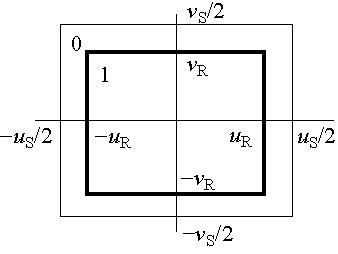
\includegraphics[scale=1.0]{04_digitalizace/images/img_4_3.pdf}
    \end{center}
    \caption{Frekvenční charakteristika obdélníkového rekonstrukčního filtru.}
    \label{img:4_3}
\end{figure}

Abychom mohli vztahu \eqref{eq:4_15} prakticky využít, zbývá ještě určit impulzovou charakteristiku \textit{r}(\textit{x},\textit{y}) rekonstrukčního filtru \eqref{eq:4_14}. Zpětnou Fourierovou transformací získáme ze vztahu \eqref{eq:4_14} předpis

\begin{equation} \label{eq:4_16}
    r(x, y) = 4 u_\mathrm{R} v_\mathrm{R} \, \mathrm{sinc} (2 x u_\mathrm{R}) \, \mathrm{sinc} (2 y v_\mathrm{R}).
\end{equation}
Vidíme tedy, že v prostorové doméně lze rekonstrukci obrazu provést podle předpisu \eqref{eq:4_15} jako konvoluci vzorků \textit{f}$_\mathrm{I}$(\textit{k}$\Delta$\textit{x},\textit{l}$\Delta$\textit{y}) vstupního obrazu s funkcí \textrm{sinc}.

\section*{Zpřesněné modely vzorkování}

Zjednodušující předpoklady, které jsme zavedli v podkapitole \ref{sec:vzorkovani_deterministicky_popsanych_signalu}, směřovaly k tomu, abychom získali jednoduché a názorné výsledky. Přestože jsou takto získané výsledky užitečné, považujeme za nutné alespoň naznačit možné modifikace uvedeného postupu, jejichž cílem je věrnější popis skutečnosti.

\noindent \textit{Konečný obraz a konečný počet vzorků:} V předchozí podkapitole jsme předpokládali, že obraz, který vzorkujeme, je definován nad nekonečnou oblastí a že vzorkováním získáme nekonečné množství vzorků. V praxi však pracujeme s obrazy, které jsou konečné a konečný musí být také počet vzorků. Zlepšení souhlasu teoretického modelu vzorkování se skutečností by v tomto ohledu bylo možné dosáhnout zavedením vzorkovací funkce ve tvaru konečného pole Diracových impulzů

\begin{equation} \label{eq:4_17}
    s(x, y) = \sum\limits_{k=-K}^{K} \sum\limits_{l=-L}^{L} \delta(x - k\Delta x, y - l\Delta y),
\end{equation}
kde \textit{K},\textit{L} jsou meze pole. Tento postup však bohužel komplikuje další analýzu.

\noindent \textit{Obecný tvar vzorkovacího pulzu:} Až doposud jsme předpokládali, že matematickým modelem získání vzorků je součin obrazu s vzorkovací funkcí. Jako vzorkovací funkci jsme používali funkci složenou z Diracových impulzů. Obecně však mohou mít vzorkovací pulzy i jiný tvar. Jestliže je tvar pulzu popsán funkcí \textit{p}(\textit{x},\textit{y}), pak můžeme vzorkovací funkci popsat vztahem

\begin{equation} \label{eq:4_18}
    s(x, y) = \sum\limits_{k=-K}^{K} \sum\limits_{l=-L}^{L} p(x - k\Delta x, y - l\Delta y),
\end{equation}

\noindent \textit{Vzorkování integrací:} Senzory, které lze prakticky realizovat, nedokáží sejmout hodnotu v nekonečně malém bodě. Místo toho je sejmuta jakási průměrná hodnota podél citlivé plošky senzoru. Tuto skutečnost lze zohlednit tak, že jako matematický model získávání vzorků volíme integraci

\begin{equation} \label{eq:4_19}
    f_\mathrm{S}(k\Delta x, l\Delta y) = \int\limits_{k\Delta x - \alpha}^{k\Delta x + \alpha} \int\limits_{l\Delta y - \beta}^{l\Delta y + \beta} f_\mathrm{I}(x, y) p( x - k\Delta x, y - l\Delta y)\,dx\,dy,
\end{equation}
kde $\alpha$,$\beta$ jsou poloviny délek stran snímací plošky senzoru, kterou si zde představujeme jako obdélník. Rozměry snímací plošky při tom předpokládáme menší, než je teoretická vzdálenost vzorkovacích bodů. Funkce \textit{p}(\textit{x},\textit{y}) popisuje průběh citlivosti plošky. Vzorkování integrací má značný význam. To proto, že ať chceme či nechceme, vždy k němu v praxi do určité míry dochází. Ukažme proto další možnou interpretaci vztahu \eqref{eq:4_19}. Záměnou proměnných převedeme výraz \eqref{eq:4_19} na tvar

\begin{equation} \label{eq:4_20}
    f_\mathrm{S}(k\Delta x, l\Delta y) = \int\limits_{- \alpha}^{\alpha} \int\limits_{- \beta}^{\beta} f_\mathrm{I}(k\Delta x - a, l\Delta y - b)p(-a, -b)\,da\,db.
\end{equation}

Vztah \eqref{eq:4_20} je výpočtem konvoluce funkcí \textit{f}$_\mathrm{I}$(\textit{x},\textit{y}), \textit{p}($-$\textit{x},$-$\textit{y}). Výsledek konvoluce použijeme jen v bodech \textit{k}$\Delta$\textit{x}, \textit{l}$\Delta$\textit{y} (mimo tyto body předpokládáme funkční hodnotu \textit{f}$_\mathrm{S}$ rovnu 0). Můžeme proto psát

\begin{equation} \label{eq:4_21}
    f_\mathrm{S}(x, y) = \left[ f_\mathrm{I}(x, y) * p(-x, -y) \right] \sum\limits_{k=-\infty}^{\infty} \sum\limits_{l=-\infty}^{\infty} f_\mathrm{I} \delta( x - k\Delta x, y - l\Delta y).
\end{equation}

Výraz \eqref{eq:4_21} ukazuje, že vzorkování integrací má stejný účinek, jako kdybychom provedli konvoluci vstupního obrazu \textit{f}$_\mathrm{I}$(\textit{x},\textit{y}) se vzorkovací funkcí \textit{p}($-$\textit{x},$-$\textit{y}) a pak následně provedli vzorkování polem Diracových impulzů. Jak vyplývá z vlastnosti (2.28a) Fourierovy transformace, realizuje konvoluce obrazu se vzorkovací funkcí filtraci obrazu. Ta může být někdy nežádoucí, protože způsobuje degradaci obrazu. Jindy může být naopak vítaná - např. tehdy, jestliže vzorkování obrazu probíhá na nižší frekvenci, než odpovídá Nyquistovu teorému, a je proto nutné potlačit v obraze vyšší frekvenční složky.

\section*{Aliasing} \label{sec:aliasing}

Ve vztahu \eqref{eq:4_8} jsme ukázali, že frekvenční spektrum obrazu po vzorkování se skládá ze složek, které jsou tvořeny frekvenčním spektrem vstupního obrazu. Tyto složky se periodicky opakují ve vzdálenostech \textit{u}$_\mathrm{S}$, \textit{v}$_\mathrm{S}$ a sčítají. Zjistili jsme také, že k tomu, aby mohl být obraz úspěšně rekonstruován, je nutné, aby se jednotlivé složky spektra navzájem nepřekrývaly. Dosud jsme však neřešili otázku, co se stane v případě, že tato podmínka není splněna. Věnujme se nyní tomuto problému podrobněji. Na základě vztahu \eqref{eq:4_8} je možné spektrum obrazu po vzorkování zapsat ve tvaru

\begin{equation} \label{eq:4_22}
    F_\mathrm{S}(u, v) = u_\mathrm{S} v_\mathrm{S} \left[ F_\mathrm{I}(u, v) + F_\mathrm{Q}(u, v) \right],
\end{equation}
kde \textit{F}$_\mathrm{I}$(\textit{u}, \textit{v}) je spektrum původního obrazu a \textit{F}$_\mathrm{Q}$(\textit{u}, \textit{v}) zahrnuje všechny ty složky spektra \textit{F}$_\mathrm{S}$(\textit{u}, \textit{v}) obrazu po vzorkování, pro které je ve výrazu \eqref{eq:4_8} \textit{k} $\neq$ 0, \textit{l} $\neq$ 0 (složka \textit{k} = 0, \textit{l} = 0 je zastoupena členem \textit{F}$_\mathrm{I}$(\textit{u}, \textit{v})). Předpokládejme nyní, že se jednotlivé složky spektra navzájem překrývají (obr. \ref{img:4_4}) a že na takto vzorkovaný obraz aplikujeme rekonstrukční filtr s~frekvenční charakteristikou

\begin{equation} \label{eq:4_23} 
    R\left(u,v\right) = \left\{
    \begin{array}{cc}
    1, & \left(|u| \le u_\mathrm{S} /2\right) \cap \left(|v|\le v_\mathrm{S} /2\right) \\
    0, & \mathrm{jinak}
    \end{array}
    \right. .  
\end{equation}

Zvolený rekonstrukční filtr propouští kromě složky \textit{k} = 0, \textit{l} = 0 (užitečná složka) frekvenčního spektra také určité části složek \textit{k} $\neq$ 0, \textit{l} $\neq$ 0 (nežádoucí složky). Na obr. \ref{img:4_4} jsou přenášené části nežádoucích složek vyšrafovány. Naopak si však také můžeme povšimnout, že nejsou přenášeny některé části užitečné složky. Chyba způsobená neúplným přenesením užitečné složky způsobí rozmazání obrazu (potlačení vyšších frekvencí). Naopak chyba způsobená přenosem částí nežádoucích složek dává v obraze vzniknout novým útvarům. Tento jev nazýváme aliasing. Nechť \textit{f}$_\mathrm{ID}$(\textit{x},\textit{y}) je obraz degradovaný neúplným přenosem užitečné složky. Vznik aliasingu můžeme matematicky modelovat tak, že na obraz \textit{f}$_\mathrm{ID}$(\textit{x},\textit{y}) superponujeme chybový obraz \textit{a}(\textit{x},\textit{y}) vzniklý částečným přenosem nežádoucích složek. Je tedy

\begin{equation} \label{eq:4_24}
    f_\mathrm{R}(x, y) = f_\mathrm{ID}(x, y) + a(x, y).
\end{equation}

Chybový obraz \textit{a}(\textit{x},\textit{y}) můžeme popsat vztahem

\begin{equation} \label{eq:4_25}
    a(x, y) = \mathscr{F}^{-1} \left\{ R(u, v) F_\mathrm{Q}(u, v) \right\}.
\end{equation}

\begin{figure}[th]
    \begin{center}
        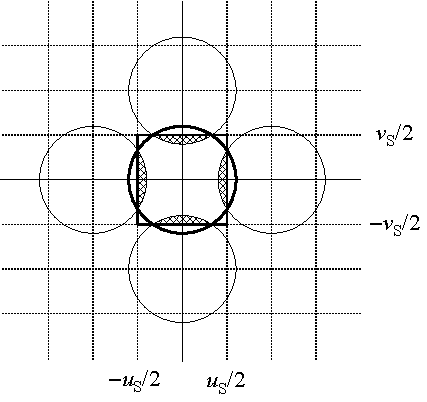
\includegraphics[scale=1.0]{04_digitalizace/images/img_4_4.pdf}
    \end{center}
    \caption{Vznik aliasingu překrýváním složek spektra vzorkovaného obrazu.}
    \label{img:4_4}
\end{figure}

Pokusme se nyní kvantifikovat míru degradace rekonstruovaného obrazu, kterou aliasing způsobí. Ke kvantifikaci použijeme stochastického přístupu. Nechť \textbf{f}$_\mathrm{I}$(\textit{x},\textit{y}) je vstupní náhodné pole a \textit{G}$_\mathrm{f_\mathrm{I}f_\mathrm{I}}$(\textit{x},\textit{y}) nechť je jeho výkonová spektrální hustota. Na míru degradace rekonstruovaného obrazu budeme usuzovat na základě energetické bilance. Energie \textit{E}$_\mathrm{I}$ vstupního obrazového pole je

\begin{equation} \label{eq:4_26}
    E_\mathrm{I} = \int\limits_{-\infty}^{\infty} \int\limits_{-\infty}^{\infty} G_\mathrm{f_\mathrm{I}f_\mathrm{I}} (u, v)\,du\,dv.
\end{equation}

Z této energie je rekonstrukčním filtrem na výstup přenášeno množství \textit{E}$_{\mathrm{IR}}$, kde

\begin{equation} \label{eq:4_27}
    E_\mathrm{IR} = \int\limits_{-u_\mathrm{S}/2}^{u_\mathrm{S}/2} \int\limits_{-v_\mathrm{S}/2}^{v_\mathrm{S}/2} G_\mathrm{f_\mathrm{I}f_\mathrm{I}} (u, v)\,du\,dv.
\end{equation}

Rekonstrukčním filtrem je na výstup ovšem také částečně přenášena energie nežádoucích složek. K určení velikosti této energie bychom měli vyšetřovat, jak do oblasti $\langle$$-$\textit{u}$_\mathrm{S}$/2, \textit{u}$_\mathrm{S}$/2$\rangle$$\times$$\langle$$-$\textit{v}$_\mathrm{S}$/2, \textit{v}$_\mathrm{S}$/2$\rangle$ každá z těchto složek přispívá. Není těžké zdůvodnit, že energie nežádoucích složek přenášená v~oblasti $\langle$$-$\textit{u}$_\mathrm{S}$/2, \textit{u}$_\mathrm{S}$/2$\rangle$$\times$$\langle$$-$\textit{v}$_\mathrm{S}$/2, \textit{v}$_\mathrm{S}$/2$\rangle$ je stejná jako energie, kterou přenáší užitečná složka mimo tuto oblast (prosíme čtenáře, aby platnost tohoto tvrzení promyslel). Energie \textit{E}A nežádoucích složek přenášená rekonstrukčním filtrem na výstup tedy je

\begin{equation} \label{eq:4_28}
    E_\mathrm{A} = E_\mathrm{I} - E_\mathrm{IR}.
\end{equation}

Relativní chybu $\epsilon_\mathrm{A}$ způsobenou aliasingem lze pak vyjádřit podílem

\begin{equation} \label{eq:4_29}
    \varepsilon_\mathrm{A} = E_\mathrm{A} / E_\mathrm{I}.
\end{equation}

K omezení jevů způsobených aliasingem můžeme použít filtrace, kterou provedeme ještě před vzorkováním. Cílem filtrace je potlačení vysokých frekvencí v obraze, čímž budou lépe zajištěny požadavky Nyquistova teorému. Obr. 4.5 znázorňuje matematický model takového postupu: Před vzorkování je zařazen filtr s frekvenční charakteristikou \textit{H}(\textit{u},\textit{v}). Rekonstrukce je provedena rekonstrukčním filtrem dle vztahu \eqref{eq:4_23}. Zařazením filtru \textit{H}(\textit{u},\textit{v}) do řetězce zpracování hrozí ovšem další degradace obrazu. Je tedy nutné zvolit takový filtr, kde omezení jevů aliasingu převažuje nad touto dodatečnou degradací.

\begin{figure}[th]
    \begin{center}
        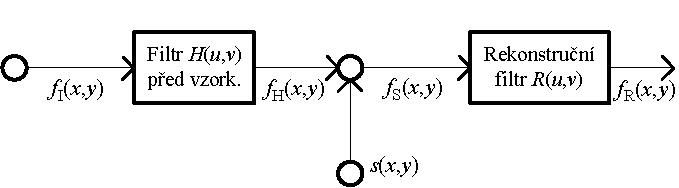
\includegraphics[scale=1.0]{04_digitalizace/images/img_4_5.pdf}
    \end{center}
    \caption{Matematický model redukce aliasingu.}
    \label{img:4_5}
\end{figure}

Nechť \textbf{f}$_\mathrm{H}$(\textit{x},\textit{y}) je náhodné pole vzniklé aplikací filtru \textit{H}(\textit{u},\textit{v}) na vstupní náhodné obrazové pole \textbf{f}$_\mathrm{I}$(\textit{x},\textit{y}) a pole \textbf{f}$_\mathrm{S}$(\textit{x},\textit{y}) nechť je pole vzniklé vzorkováním pole \textbf{f}$_\mathrm{H}$(\textit{x},\textit{y}). Označme \textit{E}$_\mathrm{H}$ celkovou energii pole \textbf{f}$_\mathrm{H}$, a dále označme \textit{E}$_\mathrm{HR}$ energii té části užitečné složky pole \textbf{f}$_\mathrm{S}$, která je propuštěna filtrem \textit{R}(\textit{u},\textit{v}) na výstup. S využitím vztahu \eqref{eq:3_27} máme

\begin{equation} \label{eq:4_30-31}
    \varepsilon_\mathrm{A} = E_\mathrm{A} / E_\mathrm{I}.
\end{equation}

Chybu $\varepsilon_\mathrm{A}$ způsobenou aliasingem a chybu $\varepsilon_{\mathrm{H}}$ způsobenou zařazením filtru \textit{H}(\textit{u},\textit{v}) lze vyjádřit vztahy

\begin{equation} \label{eq:4_32}
    \varepsilon_\mathrm{A} = (E_\mathrm{H} - E_\mathrm{HR}) / E_\mathrm{H}, \quad \varepsilon_\mathrm{H} = (E_\mathrm{IR} - E_\mathrm{HR}) / E_\mathrm{IR}.
\end{equation}

\section*{Praktické metody rekonstrukce obrazu} \label{sec:prakticke_metody_rekonstrukce_obrazu}

Úkolem rekonstrukce je získat hodnoty jasu v~bodech ležících mimo rastr, v~němž jsou k~dispozici hodnoty vzorků. Uvedený problém vzniká např. při vykreslování obrazu nebo při provádění geometrických operací s~obrazy (kapitola XXX). V podkapitole 4.1 jsme ukázali, že rekonstrukci obrazu po vzorkování lze v prostorové doméně provést konvolucí vzorků obrazu s funkcí sinc (vztahy \eqref{eq:4_15}), \eqref{eq:4_16}). Protože Fourierovým obrazem funkce sinc je ideální rekonstrukční filtr dle vztahu \eqref{eq:4_14}, je tento postup za zvolených předpokladů optimální z hlediska přesnosti rekonstrukce. Funkce sinc je však bohužel pro provádění konvoluce poněkud nepříjemná. Její hodnoty jsou téměř všude nenulové, a proto do každého bodu rekonstruovaného obrazu teoreticky přispívají všechny vzorky. Tato skutečnost vede k vysoké časové složitosti rekonstrukce. Navíc je přesné splnění předpokladů, za nichž byl ideální rekonstrukční filtr odvozen, prakticky sotva možné. V praxi se proto často používají filtry, které sice nejsou ideálními rekonstrukčními filtry, ale zato umožňují rychlý výpočet konvoluce. Rychlosti je dosahováno tím, že je impulzová charakteristika filtru nenulová jen na malé oblasti, takže do každého bodu rekonstruovaného obrazu přispívá pouze omezený počet vzorků. Frekvenční charakteristika takových filtrů se však zpravidla dosti odchyluje od charakteristiky rekonstrukčního filtru ideálního, což teoreticky vede k nižší kvalitě rekonstrukce. Uveďme několik příkladů impulzních a odpovídajících frekvenčních charakteristik častěji používaných rekonstrukčních filtrů:

\noindent 1) sinc:

\begin{equation} \label{eq:4_33a}
    r(x, y) = u_\mathrm{S} v_\mathrm{S} \sinc(u_\mathrm{S} x) \sinc (v_\mathrm{S} y),
\end{equation}

\begin{equation} \label{eq:4_33b}
    R\left(u,v\right) = \left\{
    \begin{array}{cc}
    1, & \left(|u|\le u_\mathrm{S} /2\right) \cap \left(|v|\le v_\mathrm{S} /2\right) \\
    0, & \mathrm{jinak}
    \end{array}
    \right. ;
\end{equation}

\noindent 2) čtverec:

\begin{equation} \label{eq:4_34a}
    r_0 \left(x, y\right) = \left\{
    \begin{array}{cc}
    1, & \left(-\Delta x/2<x\le \Delta x/2\right) \cap \left(-\Delta y/2<y\le \Delta y/2\right) \\
    0, & \mathrm{jinak}
    \end{array}
    \right. ,
\end{equation}

\begin{equation} \label{eq:4_34b}
    R_0 \left(u, v\right) = \Delta x \Delta y \mathrm{sinc} \, (u \Delta x) \mathrm{sinc} \, (v \Delta y);
\end{equation}

\noindent 3) trojúhelník:

\begin{equation} \label{eq:4_35ab}
    r_1 \left(x, y\right) = r_(x, y) * r_0(x, y), \quad R_1(u, v) = R_0^2(u, v);
\end{equation}

\noindent 4) zvon:

\begin{equation} \label{eq:4_36ab}
    r_2 \left(x, y\right) = r_(x, y) * r_1(x, y), \quad R_2(u, v) = R_0^3(u, v);
\end{equation}

\noindent 5) kubický B-spline:

\begin{equation} \label{eq:4_37ab}
    r_3 \left(x, y\right) = r_(x, y) * r_2(x, y), \quad R_3(u, v) = R_0^4(u, v);
\end{equation}

\noindent 6) gaussián:

\begin{equation} \label{eq:4_38ab}
    r \left(x, y\right) = \frac{1}{2 \pi \sigma^2} \exp \left[ - \frac{x^2 + y^2}{2\sigma^2}\right], \quad R(u, v) = \exp \left[ - \frac{\sigma^2( u^2 + v^2)}{2}\right]
\end{equation}

\begin{figure}[th]
    \begin{center}
        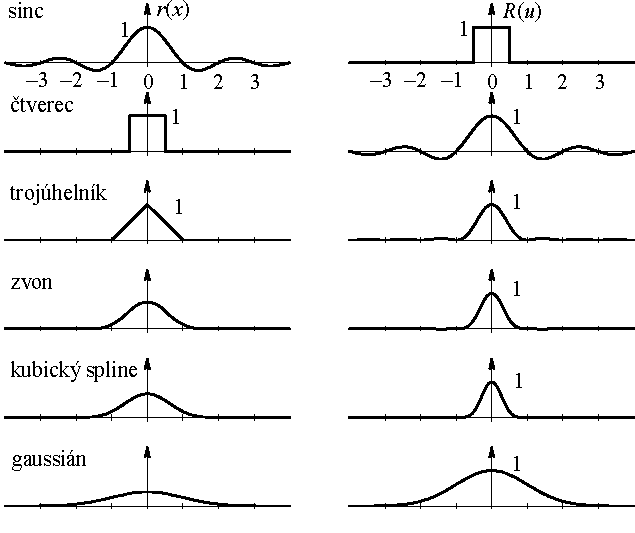
\includegraphics[scale=1.0]{04_digitalizace/images/img_4_6.pdf}
    \end{center}
    \caption{Průběhy častěji používaných rekonstrukčních filtrů ($\Delta x = u_{\mathrm{S}} = 1$).}
    \label{img:4_6}
\end{figure}

Průběhy uvedených funkcí (v jednorozměrné variantě) jsou uvedeny na obr. \ref{img:4_6}. Poznamenejme, že kvantifikaci věrnosti rekonstrukce, které lze zvoleným filtrem dosáhnout, je možné provést podobně jako v odstavci \ref{sec:aliasing} energetickou bilancí. K hodnocení může sloužit množství energie, které zvolený rekonstrukční filtr přenáší v pásmu, kde filtr ideální má frekvenční charakteristiku rovnu nule, a také rozdíl v množství energií přenášených zvoleným a ideálním filtrem v pásmu, kde filtr ideální má frekvenční charakteristiku rovnu jedné.

V~praxi se rekonstrukce dosti často provádí interpolací. Nejčastěji se používá interpolace bilineární nebo bikubické. Řekněme, že hodnota jasové funkce má být stanovena v~bodě o souřadnicích \textit{x}, \textit{y} a že $\Delta$\textit{x} = $\Delta$\textit{y} = 1. Zaveďme souřadnice $\xi$,$\eta$ (0$\leq$$\xi$,$\eta$$<$1) pomocí vztahů

\begin{equation} \label{eq:4_39}
    \xi = x - \lfloor x \rfloor, \quad \eta = y - \lfloor y \rfloor.
\end{equation}

Dále pro stručnost zápisu položme

\begin{equation} \label{eq:4_40}
    \mathbf{a} = (\lfloor x \rfloor, \lfloor y \rfloor), \quad \mathbf{b} = (\lfloor x \rfloor + 1, \lfloor y \rfloor),
\end{equation}

\begin{equation}
    \mathbf{c} = (\lfloor x \rfloor, \lfloor y \rfloor + 1), \quad \mathbf{d} = (\lfloor x \rfloor + 1, \lfloor y \rfloor + 1),\nonumber
\end{equation}

\begin{figure}[th]
    \begin{center}
        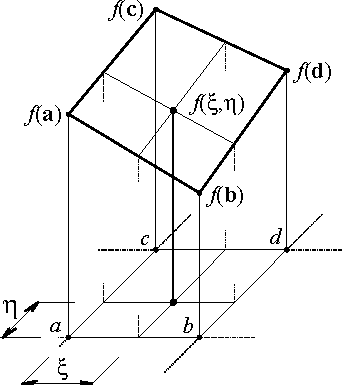
\includegraphics[scale=1.0]{04_digitalizace/images/img_4_7.pdf}
    \end{center}
    \caption{Bilineární interpolace jasu.}
    \label{img:4_7}
\end{figure}

Nechť symboly \textit{a},\textit{b},\textit{c},\textit{d} označují body, které jsou reprezentovány vektory \textbf{a},\textbf{b},\textbf{c},\textbf{d}. Bilineární interpolace je popsána následujícím vztahem (obr. \ref{img:4_7})

\begin{eqnarray} \label{eq:4_41}
    && f(x, y) = f(\lfloor x \rfloor + \xi, \lfloor y \rfloor + \eta) \\
    &=& \left[ \left( 1 - \xi\right), \xi \right] \left[
    \begin{array}{cc}
    f(\mathbf{a}) & f(\mathbf{b}) \\
    f(\mathbf{b}) & f(\mathbf{d})
    \end{array}
    \right]
    \left[
    \begin{array}{c}
    (1 - \eta) \\
    \eta
    \end{array}
    \right] \nonumber \\
    &=& (1 - \xi)(1 - \eta)f(\mathbf{a}) + \xi(1 - \eta)f(\mathbf{b}) + (1 - \xi)\eta f(\mathbf{c}) + \xi \eta f(\mathbf{d}). \nonumber
\end{eqnarray}
 
Poznamenejme, že vztah \eqref{eq:4_41} dává pro hodnotu \textit{f}(\textit{x},\textit{y}) tentýž výsledek jako konvoluce s~filtrem \textit{r}1(\textit{x},\textit{y}) dle vztahu \eqref{eq:4_35ab}. Vztah \eqref{eq:4_41} má ovšem velmi názornou interpretaci a také v~programech jej lze velmi snadno realizovat.

\begin{figure}[th]
    \begin{center}
        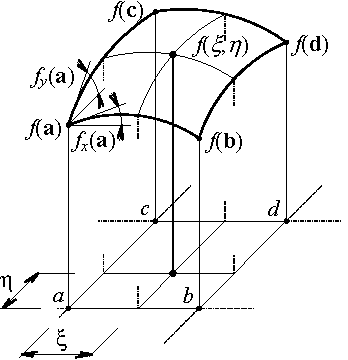
\includegraphics[scale=1.0]{04_digitalizace/images/img_4_8.pdf}
    \end{center}
    \caption{Bikubická interpolace jasu.}
    \label{img:4_8}
\end{figure}

Při vyšších nárocích na kvalitu interpolace lze požít interpolace bikubické (obr. \ref{img:4_8}). Výpočet lze provést pomocí vztahu

\begin{eqnarray} \label{eq:4_42}
    f( \lfloor x \rfloor + \xi, \lfloor y \rfloor + \eta) &=& \\
    \left[ g_1(\xi), g_2(\xi), g_3(\xi), g_4(\xi) \right] && \left[
    \begin{array}{cccc}
    f(\mathbf{a}) & f(\mathbf{c}) & f_y(\mathbf{a}) & f_y(\mathbf{c}) \\
    f(\mathbf{b}) & f(\mathbf{d}) & f_y(\mathbf{b}) & f_y(\mathbf{d}) \\
    f_x(\mathbf{a}) & f_x(\mathbf{c}) & 0 & 0 \\
    f_x(\mathbf{b}) & f_x(\mathbf{d}) & 0 & 0
    \end{array}
    \right]
    \left[
    \begin{array}{c}
    g_1(\eta) \\
    g_2(\eta) \\
    g_3(\eta) \\
    g_4(\eta)
    \end{array}
    \right]. \nonumber
\end{eqnarray}

\noindent Funkce \textit{g}$_1$, \textit{g}$_2$, \textit{g}$_3$, \textit{g}$_4$ jsou definovány následujícími vztahy (obr. \ref{img:4_9})

\begin{eqnarray} \label{eq:4_43}
    g_1(\xi) &=& 1 - 3 \xi^2 + 2\xi^3, \quad g_2(\xi) = 3\xi^2 - 2\xi^3,\\
    g_3(\xi) &=& \xi - 2 \xi^2 + \xi^3, \quad g_4(\xi) = -\xi^2 + \xi^3. \nonumber
\end{eqnarray}

\begin{figure}[th]
    \begin{center}
        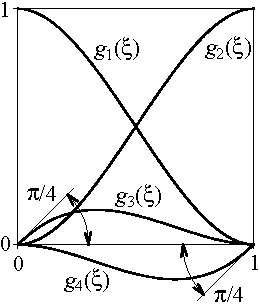
\includegraphics[scale=1.0]{04_digitalizace/images/img_4_9.pdf}
    \end{center}
    \caption{Funkce $g_1(\xi)$, $g_2(\xi)$, $g_3(\xi)$, $g_4(\xi)$.}
    \label{img:4_9}
\end{figure}

Hodnoty \textit{f}$_x$, \textit{f}$_x$ jsou hodnoty derivací (podle \textit{x} resp. podle \textit{y}) jasové funkce v~odpovídajícím bodě. Hodnoty derivací nahradíme diferencemi. Např.

\begin{eqnarray} \label{eq:4_44}
    f_x(\mathbf{a}) &=& \frac{f(\lfloor x \rfloor + 1, \lfloor y \rfloor) - f(\lfloor x \rfloor - 1, \lfloor y \rfloor)}{2},\\
    f_y(\mathbf{a}) &=& \frac{f(\lfloor x \rfloor, \lfloor y \rfloor + 1) - f(\lfloor x \rfloor, \lfloor y \rfloor - 1)}{2}. \nonumber
. \nonumber
\end{eqnarray}

Na krajích obrazu, kde nejsou hodnoty požadované vztahem \eqref{eq:4_44} k dispozici, lze použít nesymetrických diferenčních vzorců.

\noindent 

\section*{Kvantování obrazových signálů}

Při praktické reprezentaci signálů v počítači je často potřebné uchovávat jednotlivé vzorky signálu v proměnných s~omezeným rozsahem (byte, slovo atd.). V takových případech provádíme převod skutečných úrovní signálu na hodnoty, které lze v~proměnné zvoleného typu uchovávat, což nazýváme kvantováním. Na konci řetězce digitálního zpracování je naopak často potřebné obraz na základě jeho kvantované reprezentace opět zrekonstruovat tak, aby co nejlépe odpovídal obrazu teoretickému. V tomto odstavci formulujeme uvedenou úlohu poněkud podrobněji a naznačíme také její možné řešení.

\begin{figure}[th]
    \begin{center}
        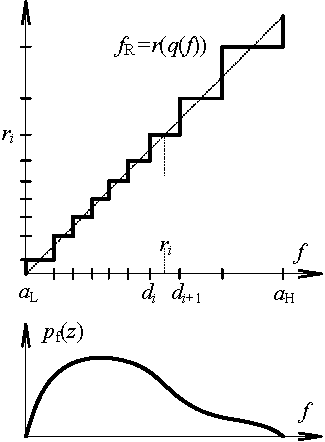
\includegraphics[scale=1.0]{04_digitalizace/images/img_4_10.pdf}
    \end{center}
    \caption{Kvantování jasu.}
    \label{img:4_10}
\end{figure}

Zvolme v~obraze nějaký libovolný bod. Nechť \textit{f} je hodnota jasu v~tomto bodě. Předpokládejme, že \textit{f} vždy nabývá reálných hodnot \textit{a}$_\mathrm{L}$ $\leq$\textit{f}$<$\textit{a}$_\mathrm{H}$, kde \textit{a}$_\mathrm{L}$,\textit{a}$_\mathrm{H}$ značí známou dolní a horní mez jasu. Proměnné, které používáme k uchovávání vzorků, nechť umožňují uložení celých čísel v rozsahu 0 až \textit{I}$-$1. Přechod od reálné hodnoty \textit{f} k~celočíselné~hodnotě \textit{i}$\in$\{0, 1,\dots, \textit{I}$-$1\} lze uskutečnit podle předpisu \textit{i} = \textit{q}(\textit{f}), který nazýváme kvantovaním. Problémem je nalézt optimální kvantovací funkci \textit{q}. Kvantovací funkce bývá obvykle zkonstruována následujícím postupem: Zvolme \textit{I}$-$1 hodnot \textit{di}, \textit{i}=1, 2, \dots, \textit{I}$-$1, které interval $\langle$\textit{a}$_\mathrm{L}$, \textit{a}$_\mathrm{H}$) rozdělí na \textit{I} podintervalů. Předpokládejme, že platí \textit{d}$_i$ $<$\textit{d}$_{i+1}$ a zaveďme dále označení \textit{a}$_\mathrm{L}$=\textit{d}$_0$, \textit{a}$_\mathrm{H}$=\textit{d}$_\mathrm{I}$. Kvantovací funkce \textit{q} zobrazuje všechny hodnoty jasu z~intervalu $\langle$\textit{d}$_i$,\textit{d}$_{i+1}$) na celé číslo \textit{i}. Problém nalezení kvantovací funkce se v~tomto případě redukuje na nalezení \textit{I}$-$1 hodnot \textit{d}$_1$, \textit{d}$_2$\textit{,} \dots, \textit{d}$_{I-1}$. Označme \textit{f}$_\mathrm{R}$ hodnotu jasu po rekonstrukci. K rekonstrukci použijeme funkce \textit{f}$_\mathrm{R}$=\textit{r}(\textit{i}). Rekonstrukční funkce \textit{r} může být v~praxi snadno realizována tabulkou. Funkce \textit{r} zobrazuje celočíselnou hodnotu \textit{i} na reálnou hodnotu \textit{r}$_i$. V úloze o kvantování hledáme pro daný rozsah \textit{I} a pro jistou třídu předpokládaných obrazových signálů hodnoty \textit{d}$_i$ a \textit{r}$_i$ tak, aby rekonstruované hodnoty jasu v jistém smyslu co nejlépe odpovídaly jasu původnímu (obr. \ref{img:4_10}).

K řešení úlohy, kterou jsme právě formulovali, můžeme použít stochastického přístupu. Považujme vzorek jasu za náhodnou proměnnou s hustotou pravděpodobnosti \textit{p}$_\mathrm{f}$(\textit{z}) (obr. \ref{img:4_10}, připomeňme, že hodnota \textit{p}$_\mathrm{f}$(\textit{z})d\textit{z} udává pravděpodobnost jevu, že jas padne do intervalu (\textit{z}, \textit{z}+d\textit{z}$\rangle$). Označme \textbf{f}, \textbf{f}$_\mathrm{R}$ náhodné proměnné popisující velikost původního a rekonstruovaného jasu. Hodnoty \textit{d}$_i$, \textit{r}$_i$ nalezneme tak, aby byla minimalizována kvantizační chyba $\epsilon = \mathrm{E}\{(\mathbf{f}_\mathrm{R}-\mathbf{f})^2\}$. Uvedený vztah vychází z~představy, že pro jasy, které se v~obraze vyskytují málo, lze tolerovat větší diferenci \textit{f}$_\mathrm{R}$ $-$\textit{f} než pro jasy, které se vyskytují často. Použitím operace střední hodnoty je zajištěno, že se diference \textit{f}$_\mathrm{R}$ $-$\textit{f} na celkové chybě podílí úměrně hustotě pravděpodobnosti jasu \textit{p}$_\mathrm{f}$. Úpravami postupně dostáváme

\begin{eqnarray} \label{eq:4_45}
    \epsilon &=& \mathrm{E} \left\{ \left[ \mathbf{f}_\mathrm{R} - \mathbf{f} \right]^2 \right\} = \mathrm{E} \left\{ \left[ r(q(\mathbf{f} )) - \mathbf{f} \right]^2 \right\} \\
    &=& \int\limits_{a_L}^{a_H} \left[ r(q(z)) - z \right]^2 p_\mathrm{f}(z)\,dz = \sum\limits_{i=0}^{I-1} \int\limits_{d_i}^{d_{i+1}} ( r_i - z)^2 p_\mathrm{f}(z)\,dz. \nonumber
\end{eqnarray}

Jestliže je počet \textit{I} úrovní dostatečně velký, můžeme často hustotu pravděpodobnosti \textit{p}$_\mathrm{f}$(\textit{z}) uvnitř jednoho kvantovacího intervalu $\langle$\textit{d}$_i$ , \textit{d}$_{i+1}$) považovat za konstantní, a to \textit{p}$_\mathrm{f}$(\textit{r}$_i$), protože zajisté bude \textit{d}$_i$ $\leq$ \textit{r}$_i$ $\leq$ \textit{d}$_{i+1}$. Ze vztahu \eqref{eq:4_45} pak dostáváme

\begin{eqnarray} \label{eq:4_46}
    \epsilon &=& \sum\limits_{i=0}^{I-1} p_\mathrm{f}(f_i)\,dz \int\limits_{d_i}^{d_{i+1}} ( r_i - z)^2 \,dz \\
    &=& \frac{1}{3} \sum\limits_{i=0}^{I-1} p_\mathrm{f}(r_i) \left[ (d_{i+1} - r_i )^3 - (d_t - r_i)^3 \right]. \nonumber
\end{eqnarray}

Z podmínky minima $\frac{\partial \epsilon}{\partial r_i} = 0$ stanovíme

\begin{equation} \label{eq:4_47}
    r_i = \frac{d_{i+1} + d_i}{2}.
\end{equation}

Dosazením vztahu \eqref{eq:4_47} do \eqref{eq:4_46} vyjde

\begin{equation} \label{eq:4_48}
    \epsilon = \frac{1}{12} \sum\limits_{i=0}^{I-1} p_\mathrm{f}(r_i)(d_{i+1} + d_i)^3.
\end{equation}

Optimální hodnoty úrovní \textit{d}$_i$ lze nalézt minimalizací hodnoty $\epsilon$. Řešení této optimalizační úlohy je poněkud nepříjemné. V (Pratt 78) se jako přibližné řešení uvádí vztah

\begin{equation} \label{eq:4_49}
    d_i = \frac{(a_\mathrm{H} - a_\mathrm{L} \int\limits_{a_\mathrm{L}}^{a_i}) \left[ p_\mathrm{f}(z)\,dz\right]^{-1/3}}{\int\limits_{a_\mathrm{L}}^{a_\mathrm{H}}) \left[ p_\mathrm{f}(z)\,dz\right]^{-1/3}} + a_\mathrm{L}, \,\,\,\mathrm{kde} \,\,\, a_i = \frac{i(a_\mathrm{H} - a_\mathrm{L})}{I} + a_\mathrm{L}.
\end{equation}

Ze vztahu \eqref{eq:4_49} je zřejmé, že jestliže je rozdělení pravděpodobnosti rovnoměrné, vychází také rozhodovací úrovně \textit{d}$_i$ rozmístěny pravidelně.

Komplikace nastávají v případě, kdy je počet kvantovacích úrovní malý, takže hustotu pravděpodobnosti na kvantovacím intervalu nelze považovat za konstantní. V takovém případě není možné provést zjednodušení použité ve výrazu \eqref{eq:4_46}, ale je nutné pracovat s výrazem \eqref{eq:4_45}. Za povšimnutí stojí také problém kvantování v~barevných obrazech. Jak víme, je barva často reprezentována trojicí \textit{R},\textit{G},\textit{B} intenzit základních barevných složek. Vlivem kvantování intenzity barevných složek může u barevných obrazů dojít k~nepřesnostem nejen v~intenzitě, ale i v~barevném odstínu.
